\chapter{基于二阶段架构的新闻长文本阅读理解}
% 摘要
长文本机器阅读理解是指,在给定一段长文本的情况下,让模型回答指定问题。
尽管基于Transformer的模型取得了很好的成果,但它们中大多数模型由于时间开销的问题,并不善于处理长序列。
一般来说,滑动窗口是其中一个合适的解决方案。这种方法将文章等分成多个片段,针对每个文本片段独立预测答案,而不考虑文本片段的上下文关系。
然而,这种方法缺乏上下文之间的远距离依赖,这会严重损坏模型性能。
为了解决这个问题,本文提出了一个专门针对长文本阅读理解的两阶段方法ThinkTwice。
ThinkTwice解决长文本阅读理解的过程主要分为两个步骤:首先检索出最终答案最有可能位于的若干个文本片段;再从这些精简后的文本片段中抽取最终的答案片段。
本章在NewsQA数据集上进行了实验。实验结果表明,ThinkTwice可以从长文本当中捕获到最具有信息含量的文本片段。
同时,ThinkTwice与现有的基线模型相比,获得了相当大的性能提升。

\section{引言}
% 绪论
机器阅读理解\cite{hermann2015teaching},旨在针对给定文本,教机器学习回答问题。这项技术一直是自然语言处理领域的最前沿研究之一。
预训练语言模型由于其多层Transformer架构以及自注意力机制\cite{vaswani2017attention},已经取得了优异的成果。

现有的机器阅读理解系统(也包括其他的自然语言处理系统)尽管在短文本领域中取得了成功,但由于预训练语言模型所能容纳的文本长度限制\footnote{例如,BERT的最大位置词嵌入长度为512.},这些系统依然不善于有效的处理长序列。
同时,如果仅仅是增加输入长度,模型的复杂度($O(n^2)$)也将呈现平方级的增长,这会导致出现维度爆炸现象。

最直观的处理方法有截断\cite{rajpurkar2016squad,xie2019unsupervised}和滑动窗口\cite{joshi2019bert}两类。
前者将长文本截断为模型所能接受的长度,而后者将文章划分为若干个固定长度的片段,并对每个片段预测答案。
这两种方法都存在问题,它们舍弃了部分文本,或者丢弃了关键的上下文信息。
由于这些棘手的问题都是由于时间和空间的高复杂度带来的,另一类研究方法主张简化Transformer架构\cite{beltagy2020longformer,zaheer2020big,ding2020ernie}。
然而,这些方法由于自身存在的问题,很少应用到现实世界中。

收到人类阅读行为的启发,本章提出了一种叫做ThinkTwice的二阶段方法来解决长文本阅读理解中的挑战。
ThinkTwice主张将长文本压缩为短文本。
想象一下,当一个人带着疑问去阅读一篇长文本时,他首先会无意识的选择一些跟给定问题相关的文本片段,然后在大脑中对这些信息进行整理;然后这些文本片段将被灌输到它的工作记忆\cite{atkinson1968human}中,从而推理出答案。
遵循这种人类的行为,ThinkTwice使用了一个检索器来过滤和压缩大量文本信息,以及使用一个阅读器来实现问答的功能。
此外,该方法还使用了一个分段模块来为长文本进行分段,以及一个融合模块来整合检索得到的关键信息。

本章在NewsQA数据集\cite{trischler2016newsqa}上评估和验证了提出的方法ThinkTwice,该数据集的文本通常比较长,并且是新闻文本。
实验结果表明,相较于一些基线模型\cite{devlin2018bert,joshi2020spanbert,tay2018densely},ThinkTwice实现了重要的提升。
特别的,该方法通过在第一阶段检索出一些具有信息量的段落,从而实现了可观的性能提升,这极大的提升了第二阶段推理的准确性。

本章的贡献主要如下:

1.本章在长文本阅读理解领域中提出了一种全新的方法ThinkTwice,它长文本压缩成短文本片段,取代了先前直接对长文本进行处理的方法。

2.实验结果证明,对长文本阅读理解数据集NewsQA\cite{trischler2016newsqa},该方法ThinkTwice在四个主要的预训练语言模型\cite{devlin2018bert,liu2019roberta,lan2019albert,joshi2020spanbert}中都取得了可观的性能提升。

\section{基于二阶段架构的新闻长文本阅读理解}
图~\ref{fig:3-1}~展示了ThinkTwice的架构,它由四个基本模块组成:
1)一个分段器,将给定文章切割为更短的文本片段;
2)一个检索器,筛选出与给定问题最相关的一些文本片段;
3)一个融合器,将筛选出的文本片段根据原始顺序进行整合;
4)一个阅读器,阅读给定问题和融合后的文本片段,从而预测出最终答案。

\begin{figure}[htbp]
    \centering
        % 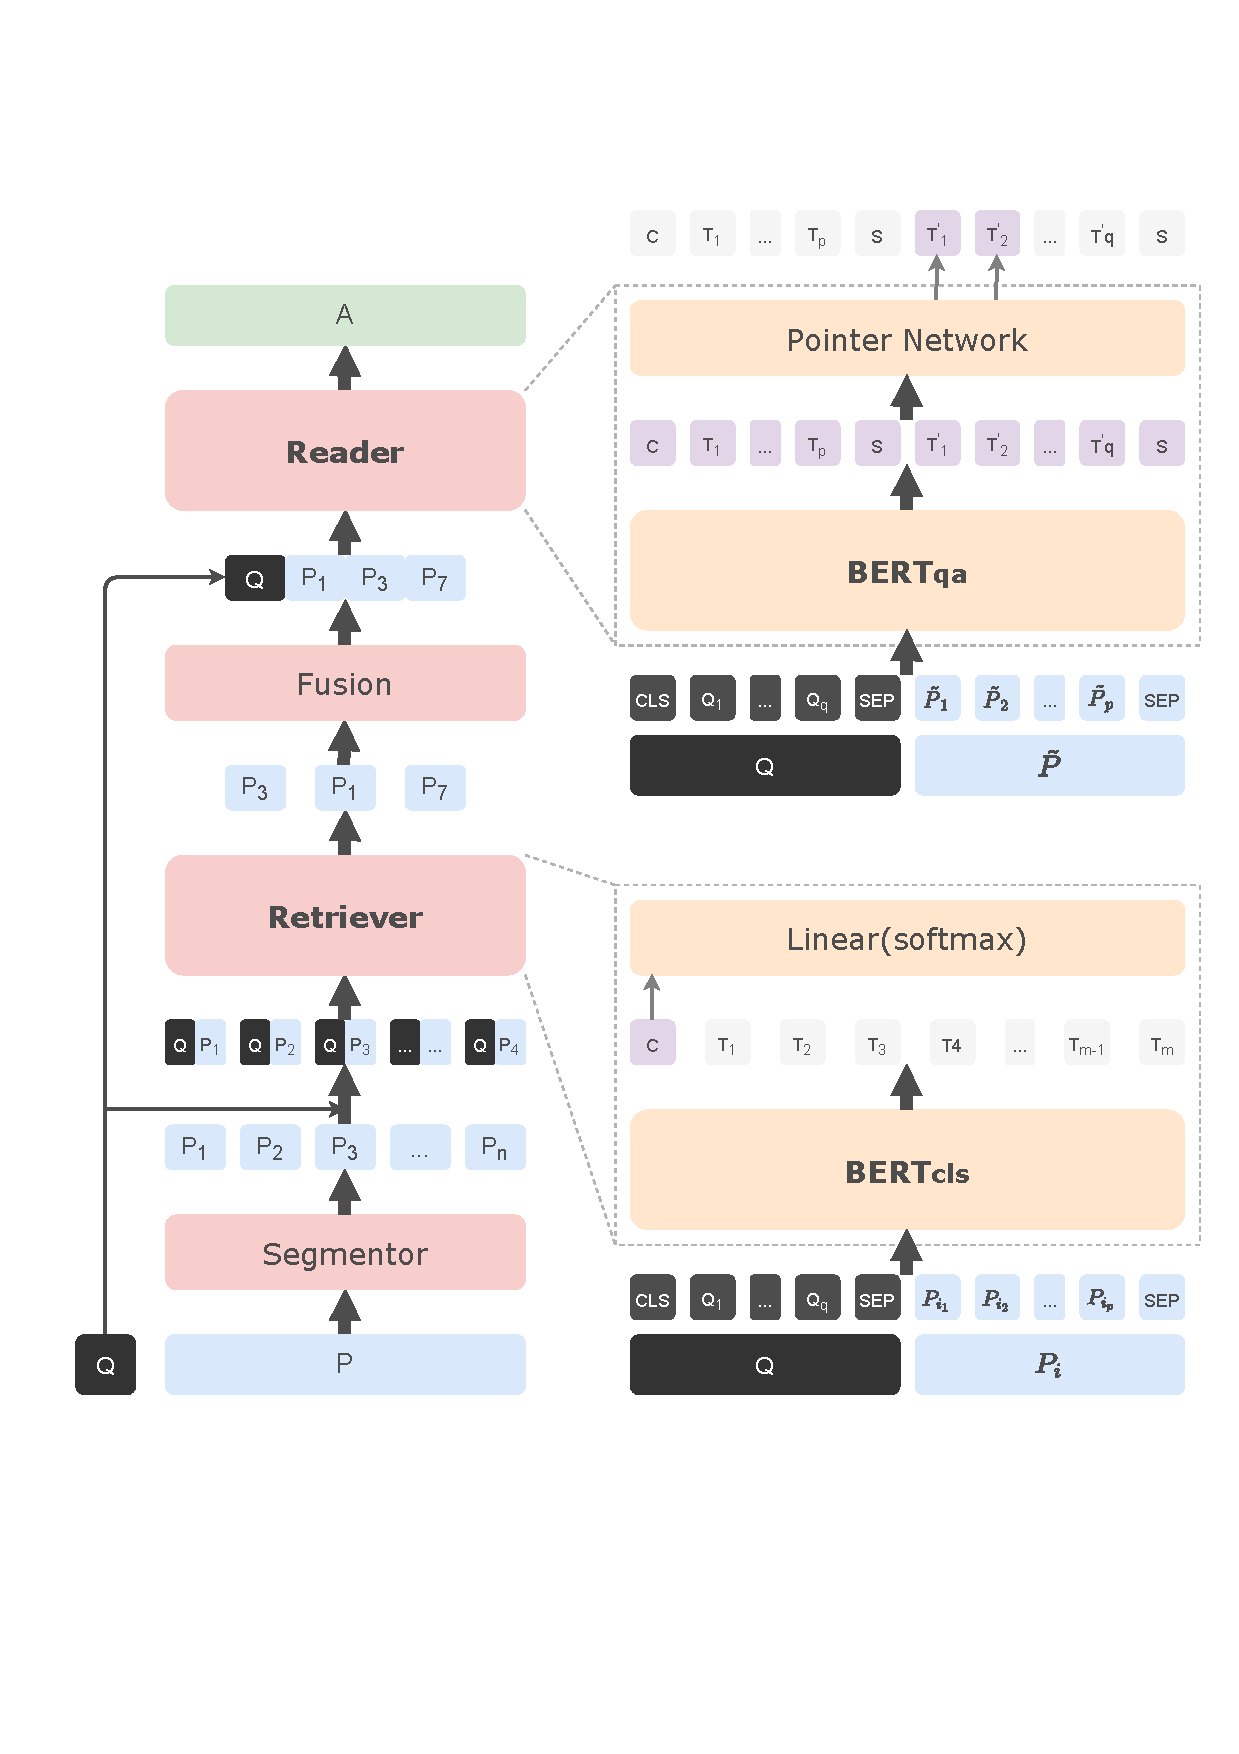
\includegraphics [width=0.8\textwidth] {figure/3-1.pdf}
        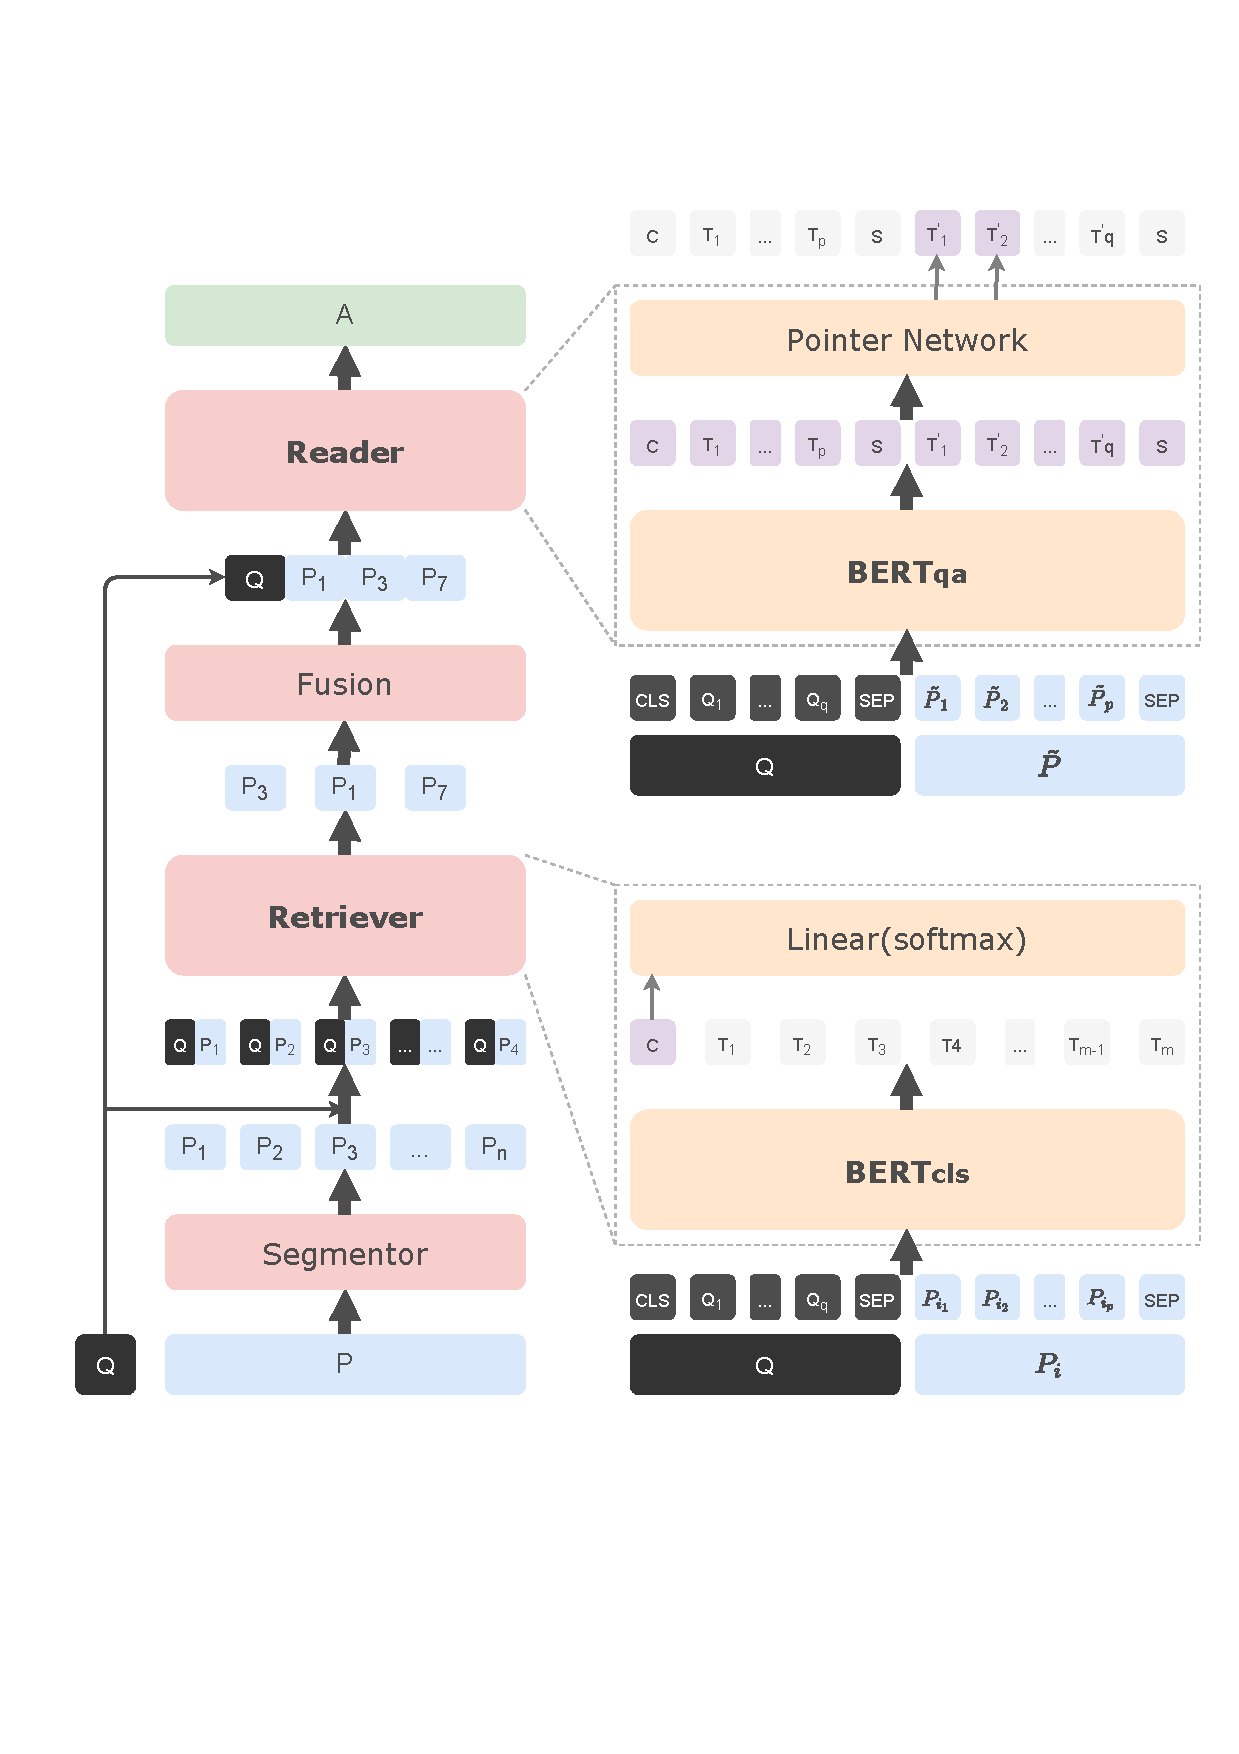
\includegraphics[scale=0.6]{figure/3-1.pdf}
    \caption{ThinkTwice的基本架构}
    \label{fig:3-1}
\end{figure}



\subsection{分段方法}
长文本阅读理解的主要挑战是,在给定文章所包含的大量知识片段当中,如何精准定位到最重要的信息。
这些文章的长度往往超过了现存神经网络模型所能容纳的最大长度(例如512个token)。
为了解决这个问题,我们为NewsQA中每篇文章的结尾增加了一个分割标记,分割之后,每个文本片段的长度被限制到60-80个token左右。
形式化的来讲,输入文本$P$被分割成文本片段$P_1,P_2,...,P_n$。

\subsection{基于预训练语言模型的段落检索器}
当一个人从大量文本当中寻找答案时,他会倾向于将与当前问题最相关的文本片段保留到大脑当中,并过滤掉琐碎的信息。
受到这种人类行为的启发,本文提出了一个基于预训练语言模型的检索器,来选择最有可能回答问题的最重要的文本片段。

检索器部分首先将问题$Q$和每个文本片段$\{P_i\}^n_{i=1}$组合成多个序列$\{x_i\}^n_{i=1}$,其中$x_i=[CLS]Q[SEP]P_i[SEP]$\footnote{[CLS]和[SPE]是特殊token。前者对于编码后的输入序列,理论上可以表示整体信息;后者主要用于分隔输入序列}。
然后,一个检索器的编码器部分,也就是预训练语言模型,用于将输入$x_i$编码成整个序列的上下文词嵌入表示$H_i$:
\begin{equation}
    H_i = BERT_{cls}(x_i).
\end{equation}

[CLS]的隐向量表示$H^{cls}_i$代表了整个序列的总体表示。然后,一层线性网络和Softmax层用于得到该序列的分类概率$\hat y_c$:
\begin{equation}
    \hat y_c=Softmax(Linear(H_i^{cls})),
\end{equation}

其中$\hat y_c$表示当前文本片段$P_i$是否包含可以回答给定问题的有效信息\cite{zhang2020retrospective}。
在训练阶段,当$P_i$包含标注答案时,“有/无答案”标签$y_{c(i)}$设为1,否则设为0。

交叉熵损失函数用于计算真实答案$y_c$和预测概率$\hat y_c$之间的损失:
\begin{equation}
    \mathcal  L_{retriever}  = -\frac{1}{n}\sum_{i=1}^{n}[y_{c(i)}\log\hat y_{c(i)}+(1-y_{c(i)})log(1-\hat y_{c(i)})].
\end{equation}

\subsection{融合方法}
上一小节通过检索器得到了输出概率值$\{\hat y_{c(i)}\}^n_{i=1}$,它可以表达每个文本片段$\{P_i\}^n_{i=1}$回答给定问题$Q$的可能性大小。
然后,通过$\hat y$的值筛选出与$Q$最相关的$k$个文本片段,并舍弃其他片段。
紧接着,被筛选出的文本片段根据它们在原文中的顺序合并成单个序列,确保整个组合文本的语义连贯性和上下文连续型。
例如,如果把$k$设成3,并且分数最高的3个文本片段分别是$P_3$,$P_1$和$P_7$。
融合器需要通过它们在原文中的相对顺序,把它们拼接在一起;对于某些可能出现的特别长的文本,直接对其进行截断即可。
所以,融合器的输出可以表示为图~\ref{fig:3-1}~中的$\tilde P=<P_1,P_3,P_7>$。

\subsection{基于与训练语言模型的阅读理解模型}
通过上述模块,已经从原始的长文本$P$中抽取得到了一段短文本$\tilde P$。
本节的阅读器模块首先将问题$Q$和上一节得到的$\tilde P$拼接成单个序列$z=[CLS]Q[SEP]\tilde P[SEP]$。
然后使用另一个预训练语言模型\cite{devlin2018bert}作为阅读器的编码器,来将输入$z$映射到一个上下文隐向量序列。
下一步,指针网略将问题相关的文本表示的答案片段的起始和结束位置进行解码:
\begin{equation}
    \mathcal L_{reader} = \frac{1}{2} CrossEntropy(\hat y_s,y_s) + \frac{1}{2} CrossEntropy(\hat y_e,y_e),
\end{equation}

其中$\hat y_s$和$\hat y_e$分别表示由阅读器解码的预测答案的起始和结束位置的概率。

在训练过程中,阅读器中使用了交叉熵损失来计算起始和结束位置的损失:
\begin{equation}
    \mathcal L_{reader} = \frac{1}{2} CrossEntropy(\hat y_s,y_s) + \frac{1}{2} CrossEntropy(\hat y_e,y_e),
\end{equation}
其中,$y_s$和$y_e$分别表示开始和结束位置的标签。
如果当前段落给出的信息不能回答问题,$y_s$和$y_e$都设为0,也就是指向$[LCS]$token。
在预测阶段,阅读器首先计算“有答案”分数$score_{has}$和“无答案”分数$score_{null}$,各自用$\hat y_s$和$\hat y_e$来表示:
\begin{equation}
    score_{has}=\max \limits_{1\le i\le j<L}(\hat y_{s}^{(i)}+\hat y_{e}^{(j)}),
\end{equation}
\begin{equation}
    score_{null}=\hat y_{s}^{(0)}+\hat y_{e}^{(0)},
\end{equation}
其中$i$和$j$表示在整个序列长度$L$内的答案位置,并且由于起始位置一定在结束位置之前,有$i$一定限制为小于$j$。
另外,鉴于序列首部的$[CLS]$不表示$\tilde P$中的任何词,$\hat y^{(0)}_s$和$\hat y^{(0)}_e$表示整个文本没有答案的概率。

接下来,通过计算$score_{has}$和$score_{null}$之间的距离来计算两者之间的距离分数$score_{dist}$,以此作为“有/无答案”的依据:
\begin{equation}
    score_{dist}=score_{null}-score_{has},
\end{equation}
\begin{equation}
    s,e=\argmax \limits_{1\le i\le j<L}(\hat y_{s}^{(i)}+\hat y_{e}^{(j)}),
\end{equation}
其中有一个阈值$\delta$,如果$score_{dist}$小于$\delta$,阅读器输出的$s$和$e$就代表了答案的起始和结束位置,否则阅读器会将该问题视为一个不可回答问题。

\section{实验及结果分析}

\subsection{实验设置}
本章在一个具有挑战的长文本阅读理解数据集NewsQA上进行实验。NewsQA包含了13,000条来源于CNN的新闻文章,有120,000条人为生成的问题答案对。
在排除20,000条标注者认为没有意义的低质量问题后,本章对剩余的数据进行了实验分析。这样NewsQA的训练/开发/测试集分别包含90,000/5,000/5,000条问题答案对。
更进一步来说,本章具体统计了每篇文章的token数量(tokens per passage, TPP)和每篇文章的段落数量(paragraphs per passage, PPP)。
TPP在训练/开发/测试集上的中位数分别为774/734/707,最大值分别为3,100/2,300/2,300。
而PPP在三个集上的中位数为18/18/17,最大值为87/63/54。

针对NewsQA数据集,存在一些长文本模型。
\begin{itemize}
    \item Match-LSTM\cite{wang2015learning}。该模型使用了两个单向的LSTM来编码问题和文章。
    \item BiDAF\cite{seo2016bidirectional}。BIDAF的核心思想是其中的双流注意力层,双流注意力分别计算上下文之于问题的注意力以及问题之于上下文的注意力。
    \item AMANDA\cite{kundu2018question}。AMANDA针对答案抽取提出了一种端到端的专注于问题的多因子注意力网络。多因子注意力编码聚合了位于多个句子中有意义的事实。
    \item DecaProp\cite{tay2018densely}。该模型把自注意力网络整合进RNN模\cite{mikolov2010recurrent}型。
    \item Longformer\cite{beltagy2020longformer}。该预训练语言模型使用了稀疏注意力矩阵,来解决序列长度的限制。
    \item CogLTX\cite{ding2020cogltx}。CogLTX架构通过判别多个句子间的相关性来识别重要句子。
\end{itemize}

本章还用两个官方指标EM和F1来计算长文本机器阅读理解的性能。EM衡量预测答案与真实答案完全匹配的比例,F1衡量预测答案与真实答案在token级的平均重叠程度。

为了证实两阶段阅读策略的有效性,本章使用了部分预训练语言模型,并通过将文章划分成多个段落的滑动窗口机制来处理长文本阅读理解问题。用到的预训练语言模型分别有:BERT\cite{devlin2018bert},RoBERTa\cite{liu2019roberta},ALBERT\cite{lan2019albert}和SpanBERT\cite{joshi2020spanbert}。
这些模型都是基于Transformer\cite{vaswani2017attention}上公开的PyTorch实现的。
在训练阶段,基础模型将学习率设为2e-5,大模型将学习率设为2e-6,热身比例设为0.1,L2权重衰减设为0.01。
批量尺寸在基础模型中是8,在大模型中是1。
对于检索器,轮次数量在基础模型中设为1,在大模型中设为2;而阅读器中这个值保持为3。
文本全部使用wordpieces\cite{wu2016google}来分词,在第一阶段最大长度设为256,第二阶段设为512.
第一阶段中进行了大量实验,用来选择$k$值\footnote{$k$值是一个超参数,表示检索器筛选出的最好的$k$个段落。}。

\begin{table}[]
    \centering
    \caption{The performances of LT-MRC models on NewsQA as well as our models' performances compared to their corresponding pre-trained language models.}
    \begin{tabular}{p{140pt}p{24pt}<{\centering}p{24pt}<{\centering}p{24pt}<{\centering}p{24pt}<{\centering}}
        %  \thickhline
         \hline
         {\bfseries Model} & \multicolumn{2}{c}{\bfseries Dev} & \multicolumn{2}{c}{\bfseries Test} \\
         & {\bfseries F1} & {\bfseries EM} & {\bfseries F1} & {\bfseries EM} \\
         \hline
         Match-LSTM~\cite{wang2015learning} & 49.6 & 34.4 & 50.0 & 34.9 \\
         BiDAF~\cite{seo2016bidirectional} & - & - & 52.3 & 37.1 \\
         AMANDA~\cite{kundu2018question} & 63.3 & 48.8 & 63.7 & 48.4 \\
         DecaProp~\cite{tay2018densely} & 65.7 & 52.5 & 66.3 & 53.1 \\
         Longformer-base~\cite{beltagy2020longformer} & 68.1 & 58.3 & 68.1 & 58.1 \\
         CogLTX~\cite{ding2020cogltx} & - & - & 70.1 & 55.2 \\
         \hline
         \hline
         BERT-base~\cite{devlin2018bert} & 65.6 & 56.3 & 65.4 & 55.2 \\
         $\ $ + ThinkTwice(descending order) & 66.6 & 57.8 & 65.8 & 55.6 \\
         $\ $ + ThinkTwice(ours) & {\bfseries 68.5} & {\bfseries58.8} & {\bfseries68.6} & {\bfseries57.7} \\
         \hline
         RoBERTa-base~\cite{liu2019roberta} & 63.7 & 53.5 & 63.2 & 53.1 \\
         $\ $ + ThinkTwice(ours) & {\bfseries67.7} & {\bfseries58.6} & {\bfseries67.7} & {\bfseries58.4} \\
         \hline
         ALBERT-base~\cite{lan2019albert} & 68.1 & 58.2 & 68.0 & 58.0 \\
         $\ $ + ThinkTwice(ours) & {\bfseries68.7} & {\bfseries59.1} & {\bfseries68.6} & {\bfseries58.8} \\
         \hline
         SpanBERT-base~\cite{joshi2020spanbert} & 67.7 & 57.1 & 67.5 & 56.2 \\
         $\ $ + ThinkTwice(ours) & {\bfseries69.9} & {\bfseries59.8} & {\bfseries69.7} & {\bfseries59.4} \\
         \hline
         BERT-large & 68.9 & 59.2 & 68.8 & 58.6 \\
         $\ $ + ThinkTwice(ours) & {\bfseries70.1} & {\bfseries59.5} & {\bfseries69.8} & {\bfseries59.4} \\
         \hline
         SpanBERT-large & 71.2 & 61.8 & 70.9 & 59.8 \\
         $\ $ + ThinkTwice(ours) & {\bfseries72.1} & {\bfseries62.2} & {\bfseries71.5} & {\bfseries61.0} \\
        %  \thickhline
         \hline
    \end{tabular}
    \label{tab:3-1}
\end{table}


\subsection{实验结果和分析}
\textbf{与现存模型相比}。表~\ref{tab:3-1}~展示了ThinkTwice与现存模型的比较结果。
该表说明,本章提出的模型在NewsQA数据集上的表现超出了现存的长文本阅读理解模型,其中在EM上提升了5.8,在F1上提升了1.4。
此外,实验结果也同样说明,实现ThinkTwice这种策略,可以在所有预训练阅读理解模型上提升性能;包括在BERT-base上的F1值提升了3.2,在RoBERTa-base上的F1提升了4.5。
然而在ALBET-base上的提升并不是很卓越。
原因可能有两点:首先,ALBERT中的句子顺序预测(sentence-order prediction)预训练任务已经解决了句子内部连贯性的问题;其次,ALBERT中实现了跨层参数共享机制,这样导致即便实现了新的策略,参数的变动也非常微小。
在其他模型上实验性能的大幅提升说明,ThinkTwice策略中的检索器精准的抽取了最重要的段落,从而让长文本压缩成合适长度的短文本,同时原始文本中最重要的信息也最大程度的保留了下来。

此外,为了观察不同融合方式对最终性能的影响,本章也尝试在BERT-base模型上用两种不同的方式来合并筛选出的文本片段。
其中一种方法将检索器抽取出的文本片段根据它们与给定问题的相关性按照降序排列并合并;另一种方法是按照先前说明的方法,以原文的顺序进行合并。
从表格~\ref{tab:3-1}~中的第8行和第9行可以发现,原始的融合方式要显著强于降序的融合方式(提升2.8),尽管用降序方式排列的模型也超出了基线模型(0.4)。
这个对比实验说明,扰乱序列顺序可能会导致上下文信息的损失。


\begin{figure}[htbp]
    \centering
    % 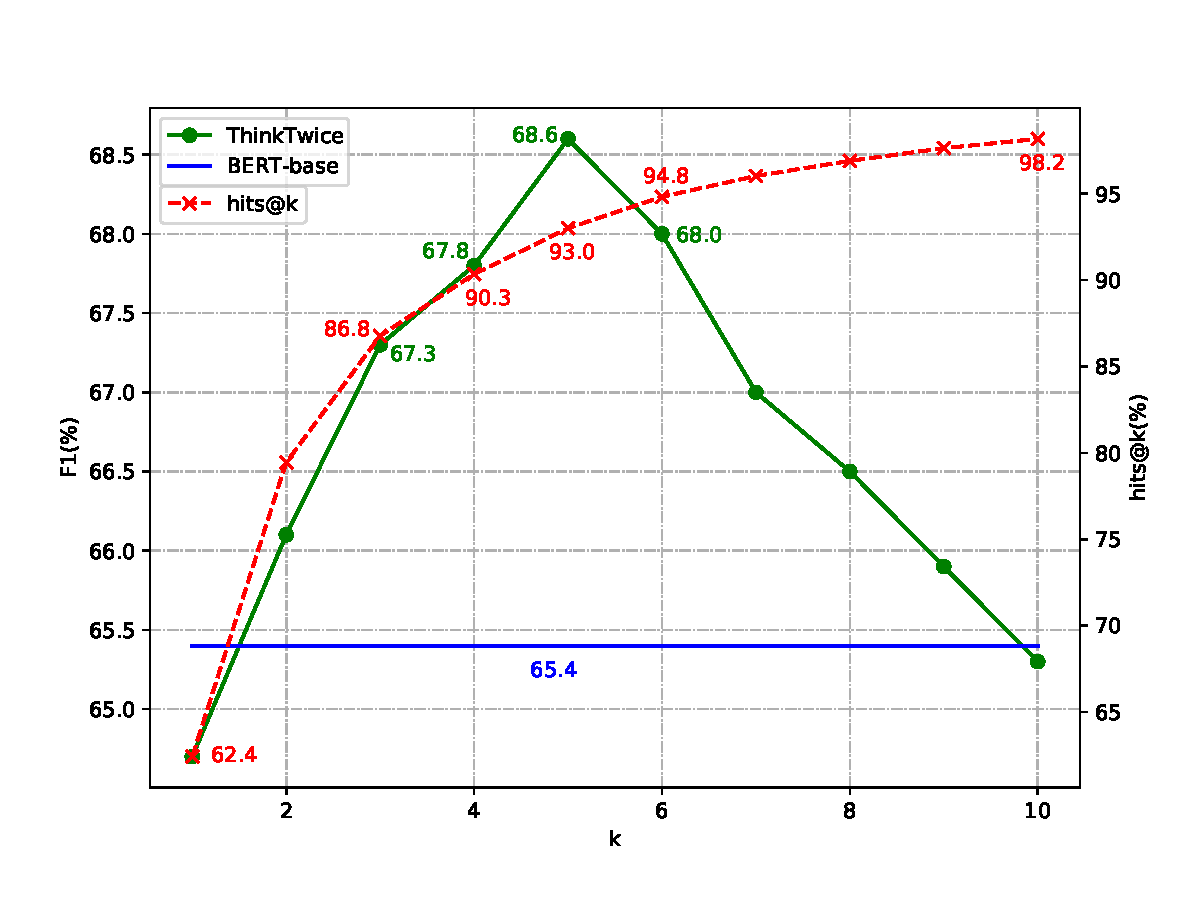
\includegraphics[width=\textwidth]{figure/3-2.pdf}
    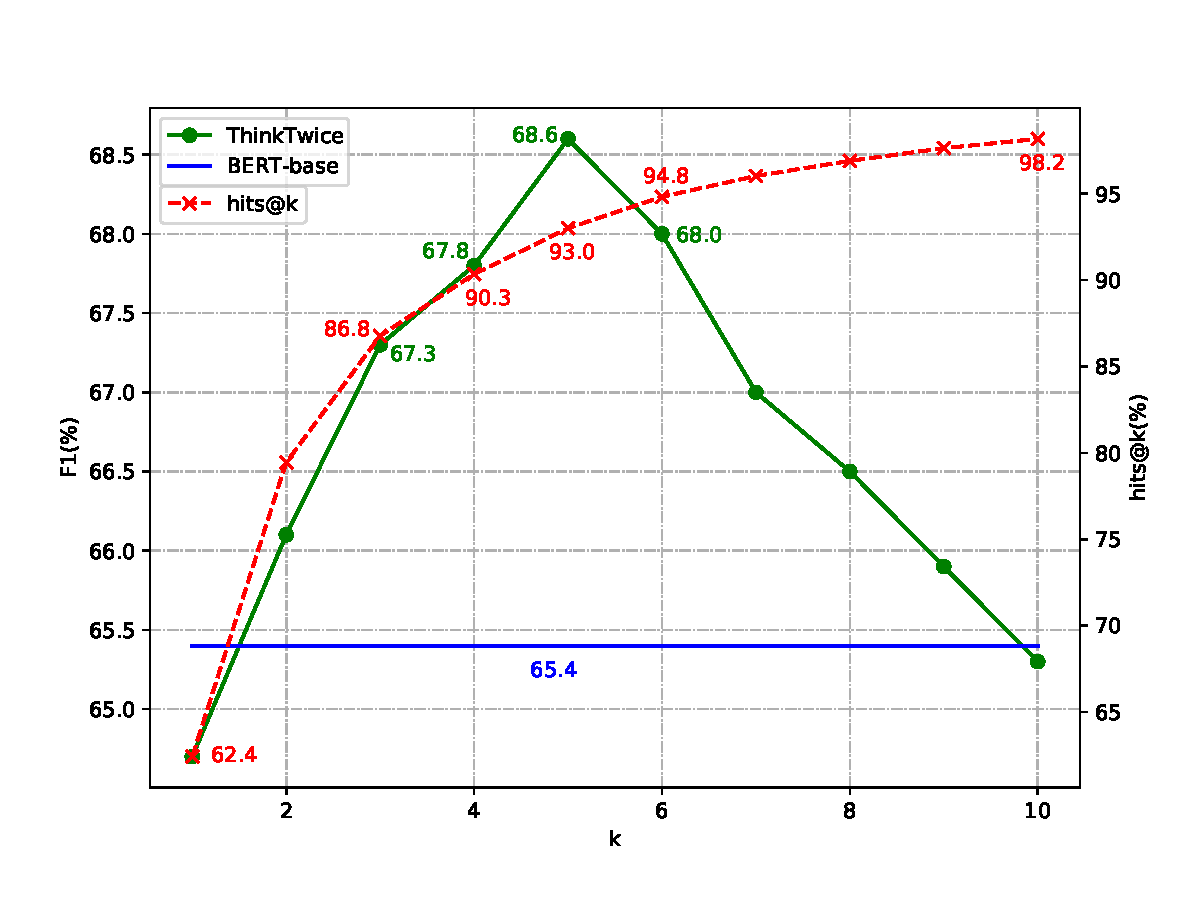
\includegraphics[scale=0.7]{figure/3-2.pdf}
    \caption{在不同$k$值情况下,检索器和ThinkTwice模型(基于BERT-base)的性能关联}
    \label{fig:3-2}
\end{figure}

\begin{figure}
    \centering
    % 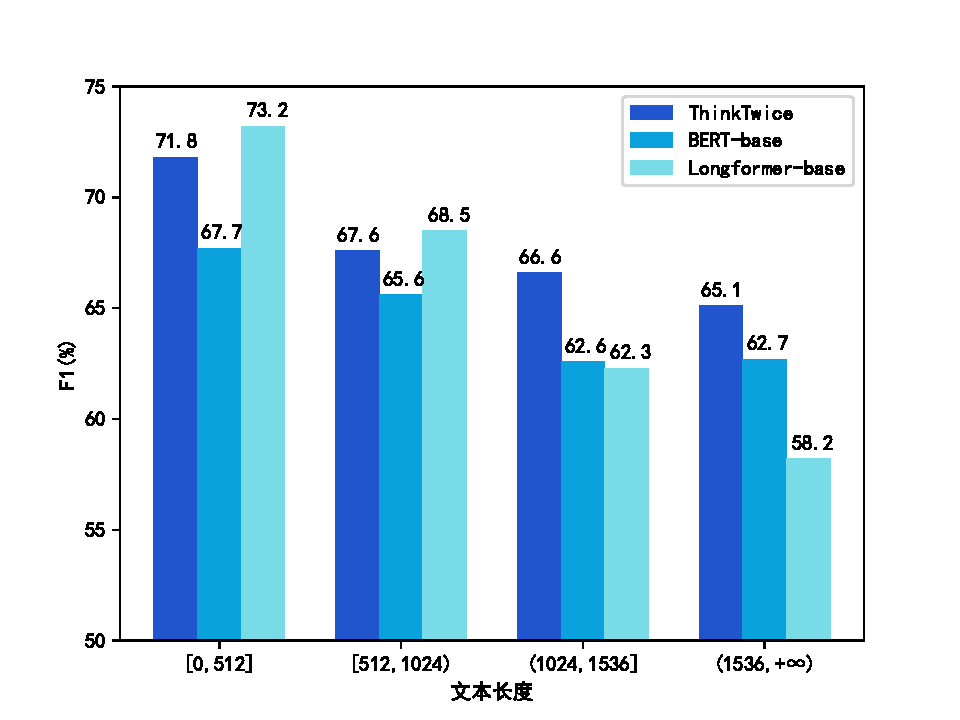
\includegraphics[width=0.7\textwidth]{figure/3-3.pdf}
    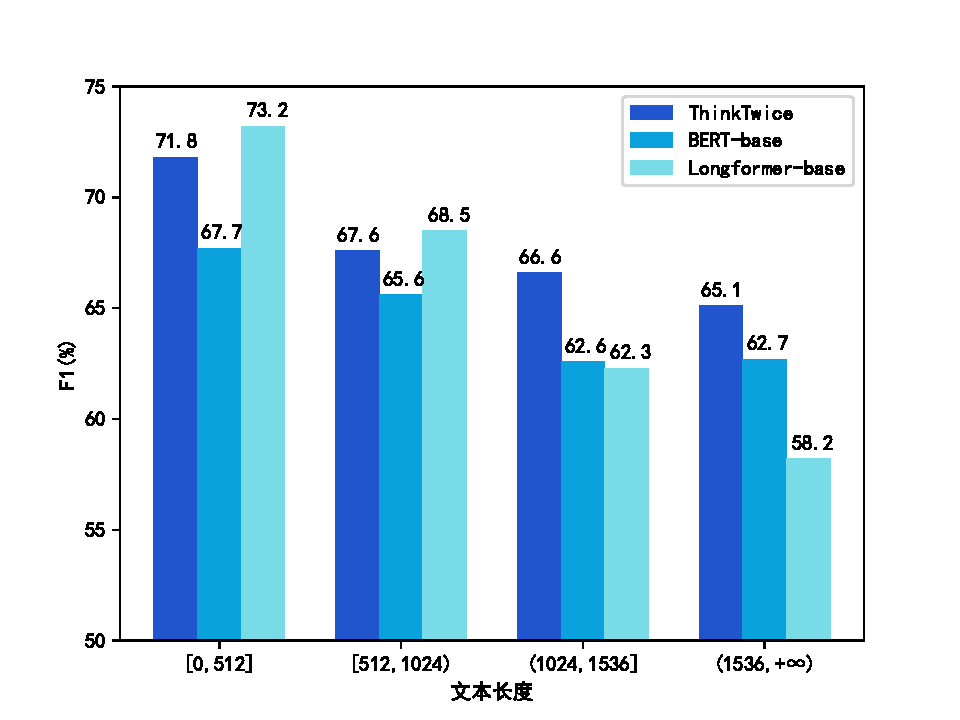
\includegraphics[scale=0.7]{figure/3-3.pdf}
    \caption{Performances of ThinkTwice, BERT-base, and Longformer-base over different text lengths. The number of samples in the four length intervals are: 1,611, 2,074, 1,089, and 210.}
    \label{fig:3-3}
\end{figure}


\noindent \textbf{段落检索}。
图~\ref{fig:3-2}~展示了检索器的不同参数配置与ThinkTwice模型之间的关系。
对于检索器,评估指标Hits@$k$(前$k$个最准确的)衡量了检索器筛选出的最好的$k$个段落是否包含真实答案。
对于ThinkTwice模型,F1评估NewsQA数据集上阅读理解模型的最终性能。
图中的红色曲线可以直观的表明,$k$值越大,Hits@$k$准确率就越高。
同样的,当$k$大于3时,检索器的该项指标也超越了90\%。
此外,当$k$等于5时,ThinkTwice模型(绿色曲线)实现了最好的性能(68.6)。
这表明,当$k$值比较小时,检索器不能召回足够多的备选段落;当$k$大于5时,更多的备选段落会面临需要搜索更大文本范围的问题。
因此,ThinkTwice在所有实验上最终将超参数$k$设为5。
本节同时也将ThinkTwice模型与相应的BERT-base阅读理解模型(蓝色曲线)进行了比较。
结果显示,当k设为2到9之间时,ThinkTwice模型表现比BERT-base好,这验证了ThinkTwice两阶段策略的有效性。

\noindent \textbf{文本长度的作用}。
为了验证ThinkTwice在长文本领域的作用,本节将多不同文本长度的测试结果与BERT-base和Longformer-base等阅读理解模型进行了比较。
值得注意的是,这里ThinkTwice模型的阅读器应用了BERT-base。
图~\ref{fig:3-3}~列出了实验结果。
可以看到,在较短的文本([0,512]和(512,1024])中,Longformer实现了最好的实验结果。其中的原因是Longformer-base继承了RoBERTa的预训练参数权重,而这些参数已经在阅读理解任务中表现的很好了。
然而,在较长的文档((1024,1536],(1536,$+\infty$))中,本章提出的ThinkTwice模型显著优于其他模型。这也证实了ThinkTwice能够准确定位到包含答案的文本片段。
此外,在较长文档的实验结果中,BERT-base也要优于Longformer-base,这表明滑动窗口机制(BERT-base)相较于直接的长文本输入(Longformer-base),也有一定优势。
最后可以发现,随着文档长度的增加,ThinkTwice模型的性能是最稳定的,特别是当文本长度大于512的时候。

\begin{table}[htbp]\scriptsize
    \centering
    \caption{NewsQA数据集上两个关于三个基线模型和CoLISA模型的预测的例子}
    \begin{tabular}{p{408pt}}
        \hline
        \multicolumn{1}{c}{\bfseries 例子1} \\
        \hline
        文章:\\
        (CNN) -- President Barack Obama spoke with Egypt's president moments after Hosni Mubarak addressed his country, telling the Egyptian that \textcolor[rgb]{1,0,0.2}{he must make good on his promises} and avoid a violent response to the thousands of protesters in the streets. (...) \\
        <译文:(...) 巴拉克·奥巴马总统在穆巴拉克发表讲话后不久与埃及总统进行了交谈,告诉埃及总统他必须履行承诺,避免对街头上万名抗议者采取暴力行动。(...) > \\
        \hline
        Token数量:2,036 \\
        \hline
        问题:\\
        What did Obama say to Mubarak? \\
        <译文:奥巴马对穆巴拉克说了什么?> \\
        \hline
        答案:\\
        he must make good on his promises \\
        <译文:他必须遵守诺言> \\
        \hline
        CoLISA预测:\\
        \textcolor[rgb]{1,0,0.2}{he must make good on his promises and avoid a violent response} (True) \\
        <译文:他必须遵守诺言并避免采取暴力行动> \\
        \hline
        BERT预测:\\
        I just spoke to him after his speech (False)
        <译文:我在他演讲结束以后跟他讲过> \\
        \hline
        ALBERT预测:\\
        It is very important that people have mechanisms in order (False) \\
        <译文:人们拥有机制非常重要> \\
        \hline
        Longformer预测:\\
        he must make good on his promises and avoid a violent response (True) \\
        <译文:他必须遵守诺言并避免采取暴力行动> \\
        \hline
        % \hline
        \multicolumn{1}{c}{\bfseries 例子2} \\
        \hline
        文章:\\
        (...) Tucked away in the verdant hills west of St. Andrews, Kingarrock Hickory Golf Course (greens fee, \$40 for nine holes and \$55 for 18) \textcolor[rgb]{1,0,0.2}{is a nine-hole, 2,022-yard country estate course that is played exclusively with antiquated equipment}. (...) \\
        <译文:(...) 坐落在圣安德鲁斯西部郁郁葱葱的山丘上,Kingarrock Hickory高尔夫球场(九洞的场地费为40美元,18洞的场地费为55美元)是一个九洞、2022码的乡村庄园球场,球场上全部使用古董设备打球。(...) > \\
        \hline
        Token数量:2,288 \\
        \hline
        问题:\\
        What is Kingarrock Hickory? \\
        <译文:Kingarrock Hickory是什么?> \\
        \hline
        答案:\\
        is a nine-hole, 2,022-yard country estate course that is played exclusively with antiquated equipment \\
        <译文:是一个九洞、2022码的乡村庄园球场,球场上全部使用古董设备打球> \\
        \hline
        CoLISA预测:\\
        \textcolor[rgb]{1,0,0.2}{a nine-hole, 2,022-yard country estate course that is played exclusively with antiquated equipment} (True) \\
        % CoLISA预测:\underline{a nine-hole, 2,022-yard country estate course that is played exclusively with antiquated equipment (True)} \\
        <译文:一个九洞、2022码的乡村庄园球场,球场上全部使用古董设备打球> \\
        \hline
        %  BERT预测:\textcolor[rgb]{0.4,0.7,0.9}{the kind of place that can change the way one thinks about golf (False)} \\
        BERT预测:\\
        the kind of place that can change the way one thinks about golf (False) \\
        <译文:一种可以改变人们对高尔夫球看法的地方> \\
        \hline
        ALBERT预测:\\
        Golf Course (True)
        <译文:高尔夫球场> \\
        \hline
        Longformer预测: \\
        Top hotel penthouses (False)
        <译文:顶级酒店顶层套房> \\
        \hline
    \end{tabular}
    \label{tab:3-2}
\end{table}

本章也执行了一个案例分析,来进一步比较NewsQA上ThinkTwice的预测结果与其他模型的区别。
结果发现ThinkTwice预测的答案与真实答案更接近。

为了验证特别长的文本上的性能,本章选取了两篇长度超过2,000词的文章作为样例,如表~\ref{tab:3-2}~所示。
在例子1中,模型需要回答奥巴马说了什么,ThinkTwice准确定位到包含最终答案的第一段段落,并且给出了奥巴马说出的合适的内容;然而BERT和ALBERT却没有像预期那样,它们分别抽取了其他段落的句子。
在例子2中,ThinkTwice也定位到了正确的段落,而BERT和Longformer表现的很糟糕。


\section{本章小结}
本章提出了一种在长文本阅读理解任务上的二阶段方法。
本章提出的ThinkTwice模型通过将长文本压缩到较短的文本形式,并准确定位到答案位置,从而解决预训练语言模型中的长度限制问题。
相关的实验结果和分析验证了该方法在长文本任务上的有效性。
该方法有一个潜在的缺陷,由检索器压缩得到的短文本可能因为缺乏先行词的原因而导致不连贯。
在未来,通过指代消解或者位置词嵌入的方式来解决这个问题将成为焦点。


